%!TEX program = xelatex
% not lualatex because of a pgf bug: https://sourceforge.net/p/pgf/bugs/384/
% makeglossaries latex-version && bibtex latex-version.aux
\documentclass[12pt, a4paper]{report}
\usepackage[T1]{fontenc}
\usepackage[english]{babel}
\usepackage{hyperref}
\usepackage{utbmcovers}
\usepackage{titlesec}
\usepackage[nottoc]{tocbibind}
\usepackage{graphicx}
\usepackage{subfig}
\usepackage[acronym]{glossaries}
\usepackage{dirtytalk}
\usepackage[toc,page]{appendix}
\usepackage{chngcntr}
\usepackage{xurl}

\titleformat{\chapter}[block]{\normalfont\huge\bfseries}{\thechapter.}{5pt}{\Huge}
\titlespacing{\chapter}{0pt}{0pt}{40pt}
% \setcounter{tocdepth}{0} % Show chapters only
% \newfontfamily\italictahomafont{Tahoma}[FakeSlant=0.4]
\newfontfamily\boldtahomafont{Tahoma}[]
\graphicspath{ {images/} }
\renewcommand*{\glstextformat}[1]{\color{black}{#1}}
\counterwithout{figure}{chapter}
\counterwithout{figure}{section}

%----------------------------------------
% utbmcovers configuration
%----------------------------------------
\setutbmfrontillustration{report_cover}
\setutbmtitle{Deep Learning for egocentric vision}
\setutbmsubtitle{ST50 thesis - P2020}
\setutbmstudent{GUETARNI Bilel}
\setutbmstudentdepartment{Computer Science department}
\setutbmstudentpathway{Image, Interaction et Réalité Virtuelle}
\setutbmcompany{Haute Ecole d'Ingénierie et de Gestion du Canton de Vaud}
\setutbmcompanyaddress{Avenue des Sports 29\\1400 Yverdon-les-Bains}
\setutbmcompanywebsite{heig-vd.ch}
\setutbmcompanytutor{PEREZ-URIBE Andres}
\setutbmschooltutor{GABER Jaafar}
\setutbmkeywords{Informatiques - Recherche - Algorithmes - Logiciel d'analyse de données - Deep Learning - Vision par ordinateur - Reconnaissance d'action - Vision égocentrique}
\setutbmabstract{
	Le deep learning a été largement utilisé dans la vision par ordinateur durant les précédentes décennies.
	Plusieurs problèmes ont étés adressés notamment la détéction d'objets, la génération de contenu, la segmentation d'image ou d'instance et une poignée d'autres.
	De nos jours, des tâches très complexes sont au coeur de la recherche académique, incluant la reconnaissance d'action ou d'activité; la différence entre ces deux tâches est très fine et nous nous concentrons ici sur la reconnaissance d'action (la différence peut être vue comme par example l'action 'prendre une fourchette' et l'activité 'cuisiner').
	\par
	Atteindre des résultats resonnables dans la reconnaissance d'action pourrait permettre de développer des systèmes de suivi de patient atteint de troubles physiques, comme des tremblements, dans leur vie de tous les jours.
	Il serait ainsi plus facile d'identifier les actions dont une personne éprouve du mal à effectuer, et ainsi conduire un processus de réhabilitation ciblée.
	Dans ce projet nous explorons comment le deep learning peut-être appliqué à la reconnaissance d'action et quel en est l'état de l'art actuel.
	Nous nous sommes concentré sur des solutions peu coûteuses en calcul puisque nous nous attendions à les implémenter sur des systèmes embarqués, e.g. téléphone mobile, NVIDIA Jetson Nano\dots
}

\makeglossaries
\newglossaryentry{ego} {name=egocentric view, description={First person view}}
\newglossaryentry{jointly} {name=jointly trained, description={Training several deep learning systems as one unique system}}
\newglossaryentry{nlp} {name=Natural Language Processing, description={Automatic process of language by computers}}
\newglossaryentry{saliency} {name=saliency, description={The property of an object to “stand-out” with respect to its surroundings}}
\newglossaryentry{synthdata} {name=synthetic-to-real domain gap, description={The unreal property of synthetic data that impacts models accuracy when trained on}}
\newglossaryentry{vanish} {name=vanishing gradient, description={Trend of the gradient to vanish during backpropagation in deep architectures}}

\begin{document}
	\makeutbmfrontcover{}

	% write table of content
	\tableofcontents{}
	
	% write glossary
	\printglossary
	
	% set paragraph indent length
	\setlength{\parindent}{15pt}
	
	\chapter*{Acknowledgements}
	\addcontentsline{toc}{chapter}{\numberline{}Acknowledgements}
	I would like to express my deep gratitude to the Haute École d'Ingénierie et de Gestion du Canton de Vaud (HEIG-VD) for receiving me during this internship and particulary to the International Office for providing me support, dedication and availability in these particular times.
	I would also like to thank the Communauté du Savoir that makes these extraterritorial cooperation possible that allow students to benefit from other universities education.
	Finally, I am particularly grateful to Mr. Andres PEREZ-URIBE and all his team, for all the advices, support and teaching they gave me.
	I adress them my very great appreciation for the assistance and the kindness they showed to me and the time they consecrated for my project.
	\chapter{Introduction}
		\section{Institut des Technologies de l’Information et de la Communication}
			The {\itshape Institut des Technologies de l’Information et de la Communication} (IICT) is the biggest research institute of the HEIG-VD university with more than 50 researchers and engineers and near 20 teachers.
			Its research is divided into software engineering, telecommunications, artifical intelligence, digital security and communication systems.
			They realize each year more than 60 projects, mostly with industrials.
			\par
			In this institut work the professor Andres PEREZ-URIBE and his team, the Intelligent Data Analysis group, on big data and intelligent data analysis.
			This team \say{works on making sense of data by developing and using data-driven models using Machine Learning approaches (including artificial intelligence, artificial life and bio-inspired approaches) as an alternative to analytical models for classification, prediction, explanation and visualization}.
			They \say{aim at providing solutions to deal with the current scenario of "data deluge" (Big Data) and to provide innovative solutions for the new ubiquitous computing world (Internet of Things and Quantified Self)}.
			They developed several applications based on intelligent systems as:
			\begin{itemize}
				\item \href{http://iict.heig-vd.ch/projets#/49/agrovision-developpement-dun-outil-de-suivi-base-sur-limagerie-aerienne-a-haute-resolution-pour-une-meilleure-gestion-agronomique-et-environnementale-de-lagriculture}{Agrovision}: an aerial image based tool for agriculture monitoring.
				\item \href{http://iict.heig-vd.ch/projets#/47/clustersitg-semantic-analysis-and-clustering-of-sitg-catalogue}{ClusterSITG}: an automatic tool for metadata organization.
				\item \href{http://iict.heig-vd.ch/projets#/43/crowdstreams-analyse-et-surveillance-en-temps-r-el-de-mobilit-la-proximit-des-grands-v-nements}{CrowdStreams}: an application for crowd analyze and monitoring.
			\end{itemize}
		\section{Internship context}
			Since the availability of huge databases, modern deep learning has been applied on several tasks with amazing performance.
			One of such tasks is action recognition.
			There have been considerable research on this topic using deep learning, but the lack of relatively large scaled datasets have limited the possibilities to develop supervised learning solutions.
			Recently, there have been considerable works to create such datasets, launching the exploration of deep learning architectures for action recognition.
			There exist a dataset, centred on actions performed in kitchen environments where the objective is to recognize a performed action (in a video) in a first person view, also called \gls{ego}.
			The purpose of this project is to create a deep learning system that is able to recognize the actions present in the dataset with the highest accuracy possible.
			\par
			\bigbreak
			We will first describe the relationship between deep learning and computer vision to understand which important part the first has became to the latter.
			Then, we'll review the egocentric action recognition state-of-the-art in the literature to describe afterwards which methods were studied.
			In a critical process, we then critic the obtained results along with an interpretation.
			Finally, we'll conclude with some observations and difficulties encountered and open some roads for future investigation.
			\par
			\bigbreak
			The code is available at: \url{https://github.com/bguetarni/Egocentric-activity-recognition}.
	\chapter{Action recognition in egocentric vision}
		\section{Deep Learning and Computer Vision}
			Deep Learning is a really successful field that is currently under innumerable investigations.
			Despite the well-known difficulties associated, numerous people jump into it every day.
			It has been successfully applied to several domains like Computer Vision, \gls{nlp} (NLP), board and video games and a raft of others.
			The first one is currently the most explored with a lot of academic research associated with huge industrial applications.
			Deep learning has revolutionized the field of computer vision by its accuracy never reached by classical algorithms.
			From the beginning, computer vision played an important role in the development of deep learning \cite{lecun1989backpropagation,lecun1998gradient,fukushima1981neocognitron}.
			However, it suffers from a major drawback, that is its need of enormous datasets.
			As the tasks tackled become more and more complex, the systems need more and more data to reach an acceptable accuracy.
			Also, most systems for computer vision are trained in a supervised learning fashion which requires data to be labeled, and for some tasks it is really hard to find such ones (even if synthetic data can be used, this still raise the problem of \gls{synthdata}).
			Moreover, the more data we have, the more computations are then needed, and we know that recent deep learning systems take a long time to train.
			\par
			Despite those drawbacks, and because several workarounds have been developed, deep learning is still seen as a powerful tool to enhance our systems.
			\subsection*{Action recognition}
				Content recognition is at the heart of the deep learning literature since the beginning. It began with numbers \cite{fukushima1981neocognitron,lecun1998gradient}, animals (e.g. cats and dogs) and more recently complex concepts such as actions.
				Human action recognition requires developing systems that can capture motion over time (sequence prediction), or systems that can recognize an action through a single frame.
				The first case has seen the emergence of new architectures as 3D convolutional networks \cite{ji20123d} and two-stream architectures \cite{sudhakaran2019lsta,wang2016temporal,ye2019two} (see \ref{twostream}).
				It is worth to notice that action recognition is itself split in two categories: first person view, also known as \gls{ego} (Figure \ref{firstperson}), and third person view (Figure \ref{thirdperson}); in this work, we focus on egocentric view action recognition.
				If we look in the literature, we'll see that egocentric vision has been neglected over third person view for a long time.
				Nonetheless, large scaled recently published datasets have exposed the egocentric view problematic and encouraged research for.
				\begin{figure}[h!]
					\centering
					\subfloat[First person.]{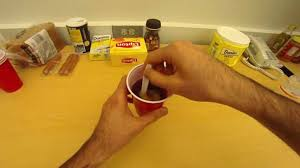
\includegraphics[width=0.4\textwidth]{firstperson.jpeg}\label{firstperson}}
					\hfill
					\subfloat[Third person.]{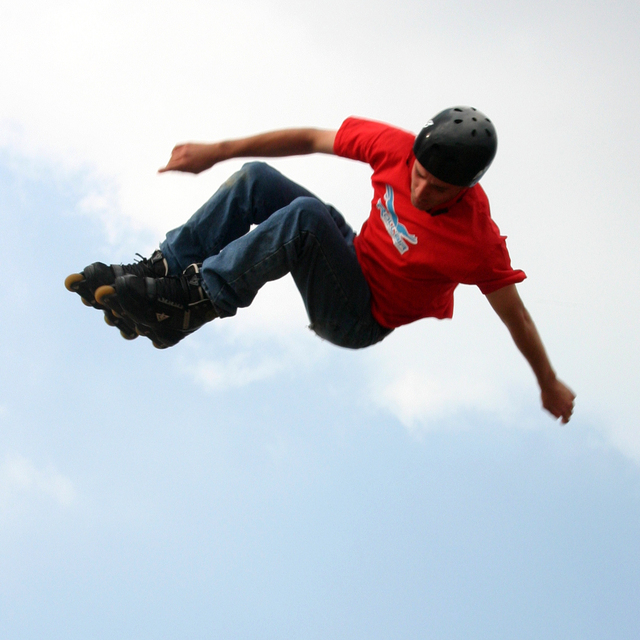
\includegraphics[width=0.4\textwidth]{thirdperson.jpg}\label{thirdperson}}
					\caption{Action views.}
				\end{figure}
				A similar task that is increasingly covered is image captioning \cite{xu2015show}, where a system try to add a caption to an image; which is related to scene understanding.
				It is easy to see that they are sensibly similar and actually, many advances that came out for image captioning are now used for action recognition (attention mechanism, recurrent neural networks).
				\subsection*{Some applications}
					Among the different applications of action recognition we find patient follow-up.
					Medical staff could use automatic egocentric action recognition to find which actions in the daily-life of a person with physical abilities disorders are the most difficult for them\footnote{Of course recognize the action is not sufficient, one should detect the disorders beforehand.}.
					And then use these analyses to conduct a targeted rehabilitation process.
					\par
					Another interesting potential of action recognition systems is video audio description, this could make all TV programs or videos accessible in audio description for blind or visually impaired people.
		\section{State-of-the-art}
			In this chapter we introduce the egocentric action recognition state-of-the-art.
			We'll describe a particular architecture that a majority of papers have focused on; for a specific reason.
			Furthermore, we'll see how different approaches, currently under investigation, taken from \gls{nlp} have achieved considerable performance.
			\subsection{Two-stream architectures}\label{twostream}
				Currently, the most used architecture for action recognition is the so-called two-stream architecture.
				It consists of two subsystems, each one processing different image modalities.
				\subsubsection{Optical flows}
					As said in the introduction of this chapter, to recognize an action it is almost necessarily to capture the motion.
					This problematic of describing motion has been extremely present in the computer vision literature and it gave rise to optical flows, sometimes also called optical flow fields.
					An optical flow is, most of the time, computed as a shift between two gray images.
					Two types of optical flows exist: {\itshape sparse} and {\itshape dense}.
					Sparse optical flows track distinct pixels among the images using feature selectors (e.g. Harris corner detector) and computes their displacement.
					On the other hand, dense optical flows are a per-pixel-motion estimate method.
					Here, we'll consider the latter one; see Appendix \ref{appendix_c} for some examples.
					There are several methods to compute dense optical flows, but the most known (and used) are the TV-L1 \cite{perez2013tv} and the Gunner Farnebäck \cite{farneback2003two} algorithms.
					\par
					Nowadays, even deep learning is considered for modeling optical flows \cite{hur2020optical}.
				\subsubsection{Literature}\label{literature}
					In \cite{wang2016temporal}, two Convolutional Neural Networks (CNN or ConvNet, they'll be used interchangeably but describe the same thing) are \gls{jointly}; rigorously speaking, one stream is trained before and used to initialize the other one before being jointly trained.
					The two-stream are identical except for the number of features expected for the input.
					The first one expect RGB images, which makes 3 features, while the second one expect stacked optical flows (2 or more features).
					Random RGB images and optical flows are drawn from the action video and fed to their corresponding CNN.
					At then end, a consensus function combines all the outputs to infer the final prediction.
					Notice that as the RGB images are processed individually, the motion can hardly be encoded by the RGB stream, in opposite with the optical flow stream.
					They also show that using RGB differences rather than stacked RGB images improves the performance.
					\par
					Yet, processing the images separately prevent the model to use the temporal correlation of the images.
					Even if we use optical flows, they describe an infinitesimal motion compared to the whole action motion.
					In \cite{ye2019two}, this idea of using the temporal correlation of the images makes use of Recurrent Neural Networks (RNN) through a ConvLSTM \cite{shi2015convolutional}.
					As originally developed, the Long Short-Term Memory (LSTM), that is discussed in \ref{lstm}, takes as input a sequence of vector and output a single vector.
					However, as we consider images it would be a waste to shrink the images into vectors for feeding them to a LSTM; because it would result in a loss of information.
					To overcome this lost of information when using LSTM, \cite{shi2015convolutional} developed the ConvLSTM cell, that allows to process images inside a LSTM.
					For this end, they replace the matrix product by a convolution.
					This simple yet effective trick create a sort of Convolutional Recurrent Neural Network.
					\par
					Later on, \cite{ye2019two} used a ResNet-101 pre-trained on ImageNet as feature extractor.
					As the others, this ConvNet is duplicated to use RGB frames and optical flows.
					The resulting feature maps of the two modes are then fused using different strategies.
					A ConvLSTM processes the sequence of fused feature maps before a final fully-connected layer.
					\par
					Last but not least, Sudhakaran et al. \cite{sudhakaran2019lsta} pointed a major difficulty to action recognition in egocentric vision that is the \say{huge variations present in the data caused by the highly articulated nature of the human body}.
					Along with this difficulty, they make the following assumption (that surely makes sense): \say{the discriminative information is often confined locally in the video frame [...] thus, not all convolutional features are equally important for recognition}.
					From these, they derive an architecture that uses a widely studied mechanism nowadays, attention.
					Simply put, they add a learnable mapping to weight the input feature maps before feeding them to the cell.
					Additionally, the output gate uses a weighted version of the cell state rather than the sequence element.
					They incorporate this mechanism with a ConvLSTM and achieve the best results to this date.
			\subsection{EPIC-KITCHENS}
				What would be deep learning without data ?
				\par
				From the very beginning, people have been struggling to push deep architectures into configurations with acceptable accuracy.
				Researchers claim that the more data is gathered for training, the likeliest the model will converge.
				However, certain problems require labels that are either complex or long to get.
				For example, image segmentation requires that every pixels of an object is labeled within its category, and this, for all objects in every images.
				On the other hand, action recognition requires to associate an action for every frame of video; we can still get around this by associating labels to a timelapse which contains an action.
				This reflects the difficulty to produce accurate and large scaled datasets for supervised learning tasks.
				\par
				For egocentric action recognition, a team of researchers have published a large scaled dataset of kitchen actions in egocentric vision: \href{https://epic-kitchens.github.io/2021}{EPIC-KITCHENS}.
				This dataset has been first published in 2018, \cite{damen2018scaling}, with approximately 40K actions using more than 55 hours of recording (EPIC-KITCHENS 55).
				Recently, a second version came out, \cite{damen2020rescaling}, with more than 90K action segments which have been extracted from 100 hours of recording (EPIC-KITCHENS 100) splitted into train (75\%), validation (10\%) and test (15\%) sets.
				Not only it contains action recognition labels, but also action detection, action anticipation and several others challenges.
				To this date, it's the biggest open egocentric action recognition dataset available.
				\par
				Each action is delimited by its frames and timesteps in the video, and is labeled with a {\itshape verb} and a {\itshape noun} (see Figure \ref{close_refrigerator}).
				\begin{figure}[h!]
					\centering
					\subfloat{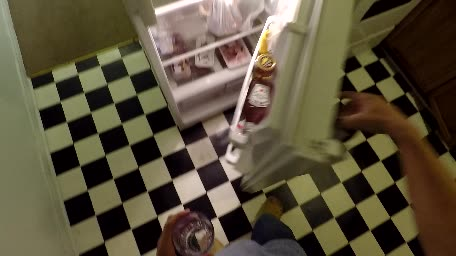
\includegraphics[width=0.55\textwidth]{close_refrigerator.jpg}\label{close_refrigerator}}
					\caption{Close ({\small verb}) the refrigerator ({\small noun}).}
				\end{figure}
				The biggest advantage of using this dataset is its natural looking data.
				The videos were recording by researchers, engineers, students and other people, in their kitchens while they were doing daily activities like: cooking, cleaning, etc.
				The resulting data have a very natural aspect which makes it suitable to train models with real world environments knowledge.
				However using a big dataset implies a finest management of the memory.% TODO: link to the RAM usage consideration
				A major drawback that natural data contained is the biased proportion between labels.
				For any activity, all actions that we do are not uniformly distributed in time.
				This is illustrated by the proportion of samples of each verb class in EPIC-KITCHENS 55 in Figure \ref{epic_55_imbalance}; the same problem occur for the noun classes.
				\begin{figure}[h!]
					\centering
					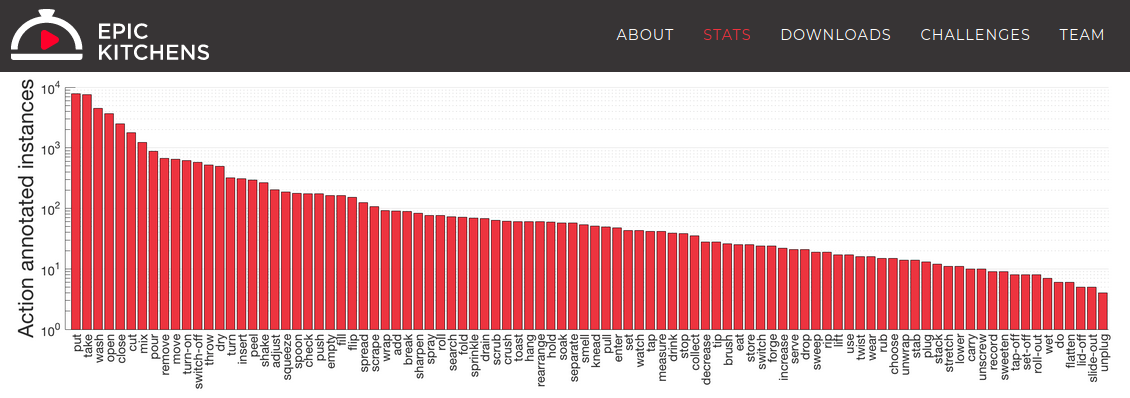
\includegraphics[width=0.85\textwidth]{EPIC-55 data imbalance.png}
					\caption{EPIC-KITCHENS 55 verbs instances.}
					\label{epic_55_imbalance}
				\end{figure}
				This class imbalance produces highly biased models toward the most represented classes in the data.
		\section{Studied methods}
			\subsection{Transfer Learning}
				As ConvNet architectures have become bigger and bigger over the past 20 years, the time and amount of computations to train these networks grew exponentially.
				Therefore, people searched for a way to reduce this training time and eventually recycle the learned knowledge, by transferring them from a domain to another.
				It's called Transfer Learning.
				The main argument of this practice is that big ConvNets layers, when trained on big dataset, will learn different features depending on their position in the architecture.
				Early layers tend to learn basic features such as: edge detectors, Gabor filters, etc.
				And the deeper we go in the architecture, the more complex these features become.
				To proof this, we provide what is called a {\itshape feature visualization} of different kernels of MobileNetV2 in Figure \ref{feature_visualization}; the reason why MobileNetV2 is given later.
				\subsubsection{Feature visualization}
					\begin{figure}[h!]
						\centering
						\subfloat[first block]{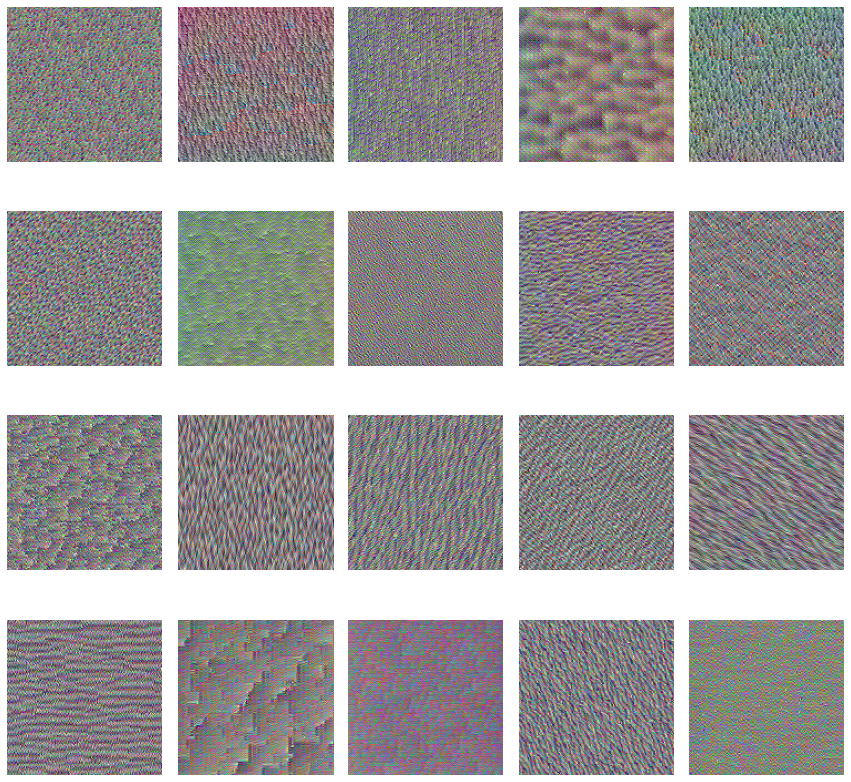
\includegraphics[width=0.45\textwidth]{kernels/block_1.png}\label{block1}}
						\hfill
						\subfloat[fourth block]{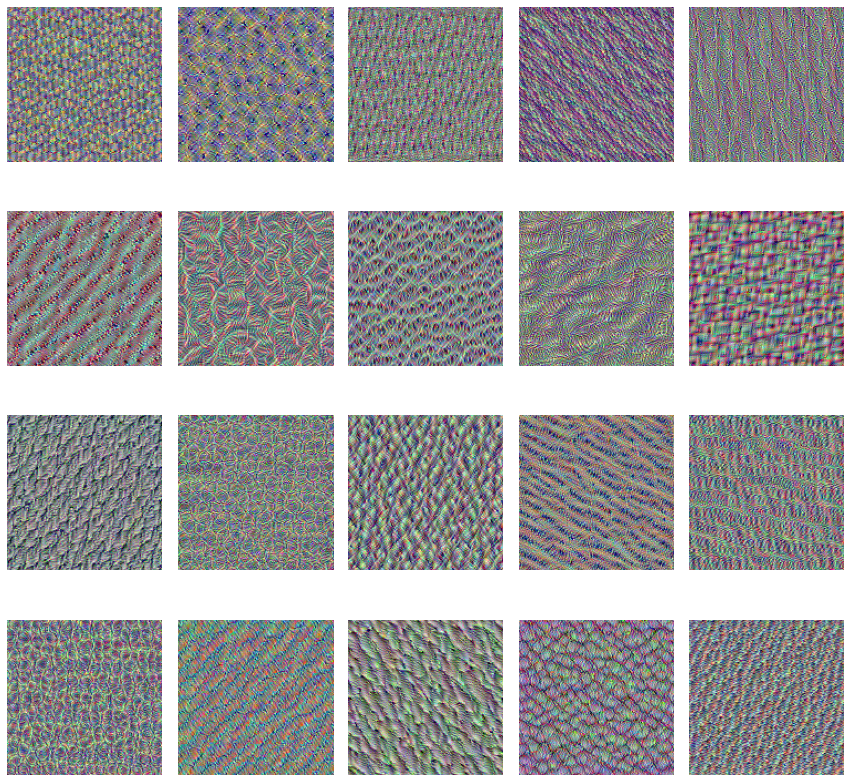
\includegraphics[width=0.45\textwidth]{kernels/block_4.png}\label{block4}}
						\vfill
						\subfloat[eighth block]{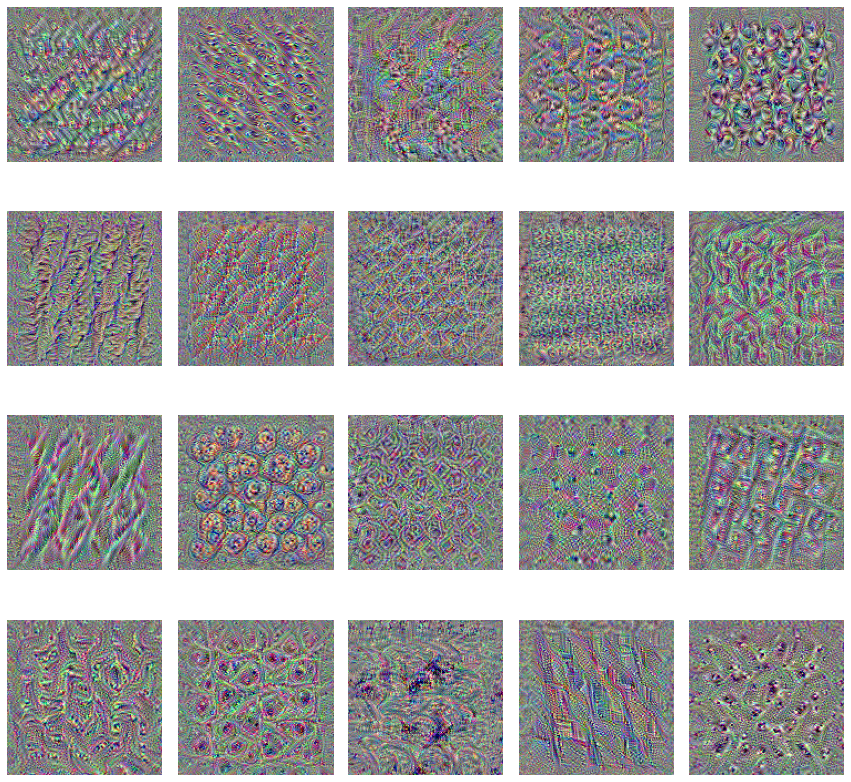
\includegraphics[width=0.45\textwidth]{kernels/block_8.png}\label{block8}}
						\hfill
						\subfloat[twelfth block]{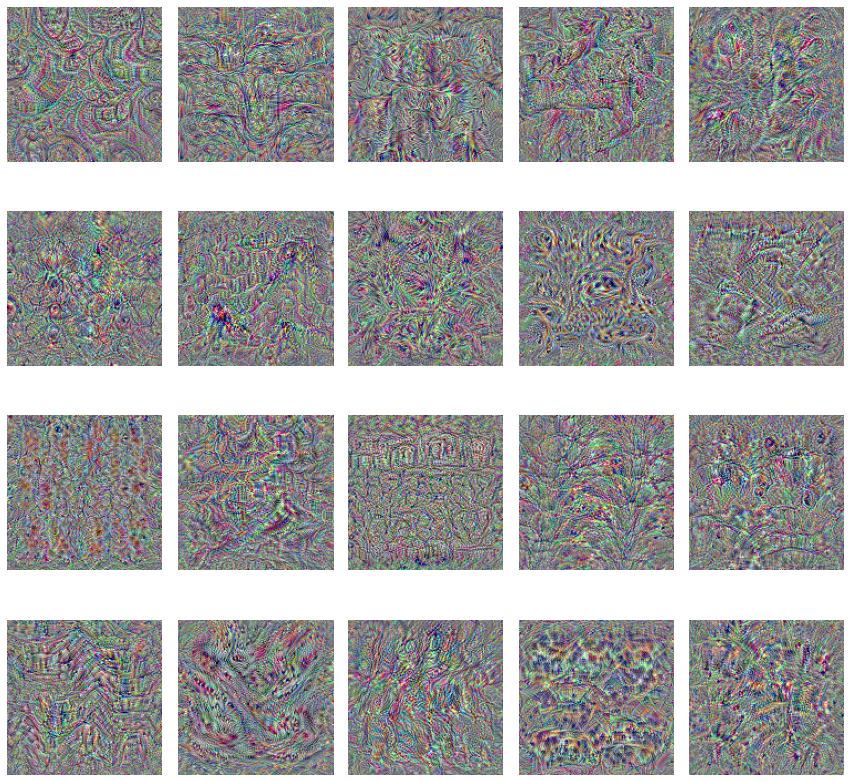
\includegraphics[width=0.45\textwidth]{kernels/block_12.png}\label{block12}}
						\caption{MobileNetV2 kernels visualization.}
						\label{feature_visualization}
					\end{figure}
					In order to provide insight of what a deep ConvNet has learned, \cite{olah2017feature} developed the feature visualization tool.
					Based on gradient ascent, this technique produces an image that will maximize the activation of a specific neuron (i.e. output of a single kernel convolution).
					We can do this because: \say{neural networks are, generally speaking, differentiable with respect to their inputs. If we want to find out what kind of input would cause a certain behavior — whether that’s an internal neuron firing or the final output behavior — we can use derivatives to iteratively tweak the input towards that goal.}
					It is useful to visualize which features a kernel, and more generally a layer, is looking for, because it provides information of the role of this layer in the architecture.
					\par
					Already before, \cite{erhan2009visualizing} applied this principle of activation maximization on different architectures trained on MNIST.
					They found that some of the resulting images \say{look like pseudo-digits}.
					When trained on natural images, the first layer filters were similar to \say{Gabor-like features}.
					Combined with other results, they suggest that \say{higher level units did indeed learn meaningful combinations of lower level features}.
				Knowing this, we can assume that the early features of a ConvNet are common features to every sort of task.
				Then we can reuse these trained models knowledge for other tasks; this is what transfer learning is all about, transfering knowledge from a domain to another.
				\par
				We provide such feature visualization for the first, fourth, eihgth and twelfth blocks, respectively, of MobileNetV2 in Figure \ref{feature_visualization}; a block is a serie of convolutions, batch normalization and activation function.
				We clearly see that in block 1 (\ref{block1}), the features are edge detectors associated with high frequency patterns.
				Deeper, in block 4 (\ref{block4}), we see more complex features, but still, they seem to be a basic combination of the previous basic features.
				And if we go even deeper, in blocks 8 and 12 (\ref{block8} and \ref{block12} respectively), the observed features are far more complex and are probably revealing what type of features one can encounter in ImageNet images.
				\par
				Based on these visuals and the previous assumptions, we first attempted to use the 9 first blocks of MobileNetV2, pre-trained on ImageNet, as feature extractor for our architectures.
				We decided to do so because the last blocks of such deep networks are too much specialized on the features present in ImageNet, that are different from those in EPIC-KITCHENS.
				We provide in appendix \ref{appendix_a}, examples of both datasets to see how different they are.
				Even if basic features are shared (edges, corners...), we thought that the high-level features to extract are not transferable from ImageNet to EPIC-KITCHENS.
				\par
				{\boldtahomafont MobileNetV2} \cite{sandler2019mobilenetv2} is a ConvNet developed with the objective to optimize the computations for edge device utilization.
				Modern deep networks have millions of parameters, and they are trained with modern technologies like GPU and TPU.
				However, embedding such networks in devices with limited computation power implies to minimize the computations, especially for real-time solutions.
				MobileNetV2 is a deep ConvNet made of several residual blocks, similarly to ResNet \cite{he2015deep}, which has been shown to help with vanishing and exploding gradient.
				It has the advantage of decomposing convolutions in two stages, first a depthwise convolution which processes one convolution per channel, and then a pointwise convolution that combines the channels.
				This reduces the computations by almost a factor of $k^{2}$, where $k$ is the kernel size.
				It contains a total of 16 blocks with an incremental number of features (24, 32, 64, ..., 320).
				The final convolution, after the last block, outputs 1280 features.
				From the beginning of the project, we intended to, if a model was successful enough, use it in an edge device with real-time predictions.
				Thus, we designed our architectures using MobileNetV2 pre-trained on ImageNet as a feature extractor.
			%\subsection{Attention}
			%	\say{Attention mechanism was proposed for focusing attention on features that are relevant for the task to be recognized} \cite{sudhakaran2019lsta}.
			%	We, humans, have the capacity to focus our {\itshape attention} into a small zone of our field of view.
			%	Thus, it allows us to process only the information we need and make abstraction of the rest.
			%	For example, while reading this, your attention is focused on these words and discard the surrounding ones even if they appear in your field of view.
			%	This way, it is easier for your mind to read.
			%	Attention was first used in NLP to help auto-encoders for translating long sentences \cite{bahdanau2014neural}.
			%	It has then been introduced in computer vision by \cite{xu2015show}, to help models for image captioning.
			%	Focusing the attention on some features requires to highlight them, so they are visually more interesting.
			%	In computer vision this can be seen as \gls{saliency} (Figure \ref{porsche}).
			%	\begin{figure}[h!]
			%		\centering
			%		\subfloat{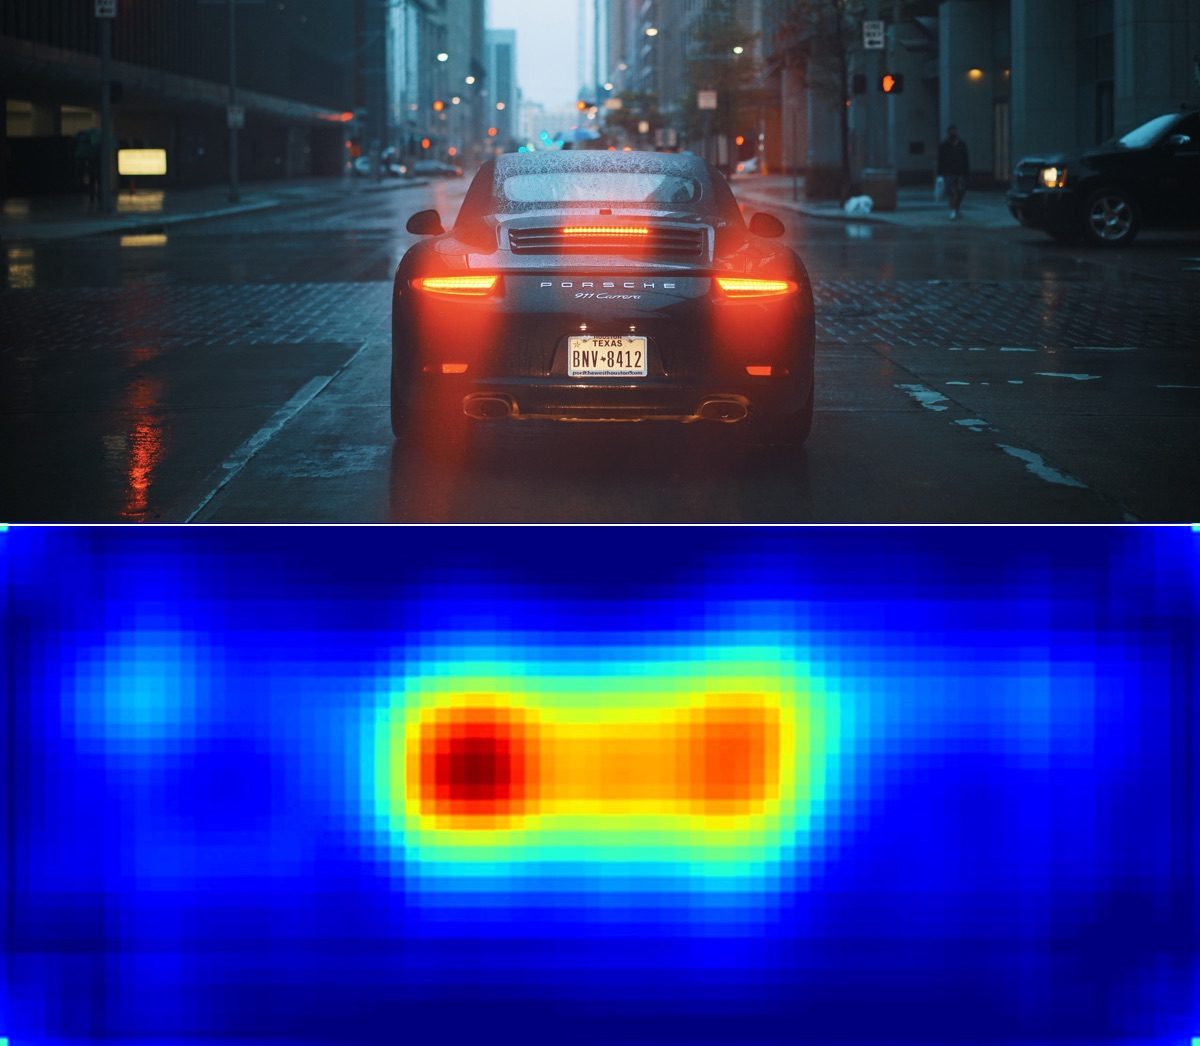
\includegraphics[width=0.4\textwidth]{porsche-saliency.jpeg}\label{porsche}}
			%		\caption{Saliency map of a car as seen by a human.}
			%	\end{figure}
			%	In deep learning, one could use weights to make some features more visible than others.
			%	In \cite{sudhakaran2018attention}, the features maps extracted by a pre-trained backbone are used as weights to encode visual attention in RGB frames; rigorously speaking, the weights are derived from a pre-classification of these features maps.
			%	Then these weighted frames go through a ConvLSTM for classification.
			%	These weighted frames are called {\itshape Spatial Attention Map}.
			\subsection{Architectures base}
				All the different architectures that we tried share a common base (drawn in Figure \ref{common_base}):
				\begin{enumerate}
					\item We draw 20 uniformly spaced RGB images ($N=20$) from the action video.
					\item Each image is fed to the pre-trained MobileNet V2.
					\item The resulting feature maps are then fed sent to a temporal processing subsystem; a spatial pooling must be applied beforehand in some cases.
					\item Finally, we use 2 fully-connected layers to output the {\itshape verb} and {\itshape noun} probability distributions.
					\item The error backpropagation is applied to the fully-connected layers and the temporal processing only (red box in Figure \ref{common_base}).
				\end{enumerate}
				\begin{figure}[h!]
					\centering
					\subfloat{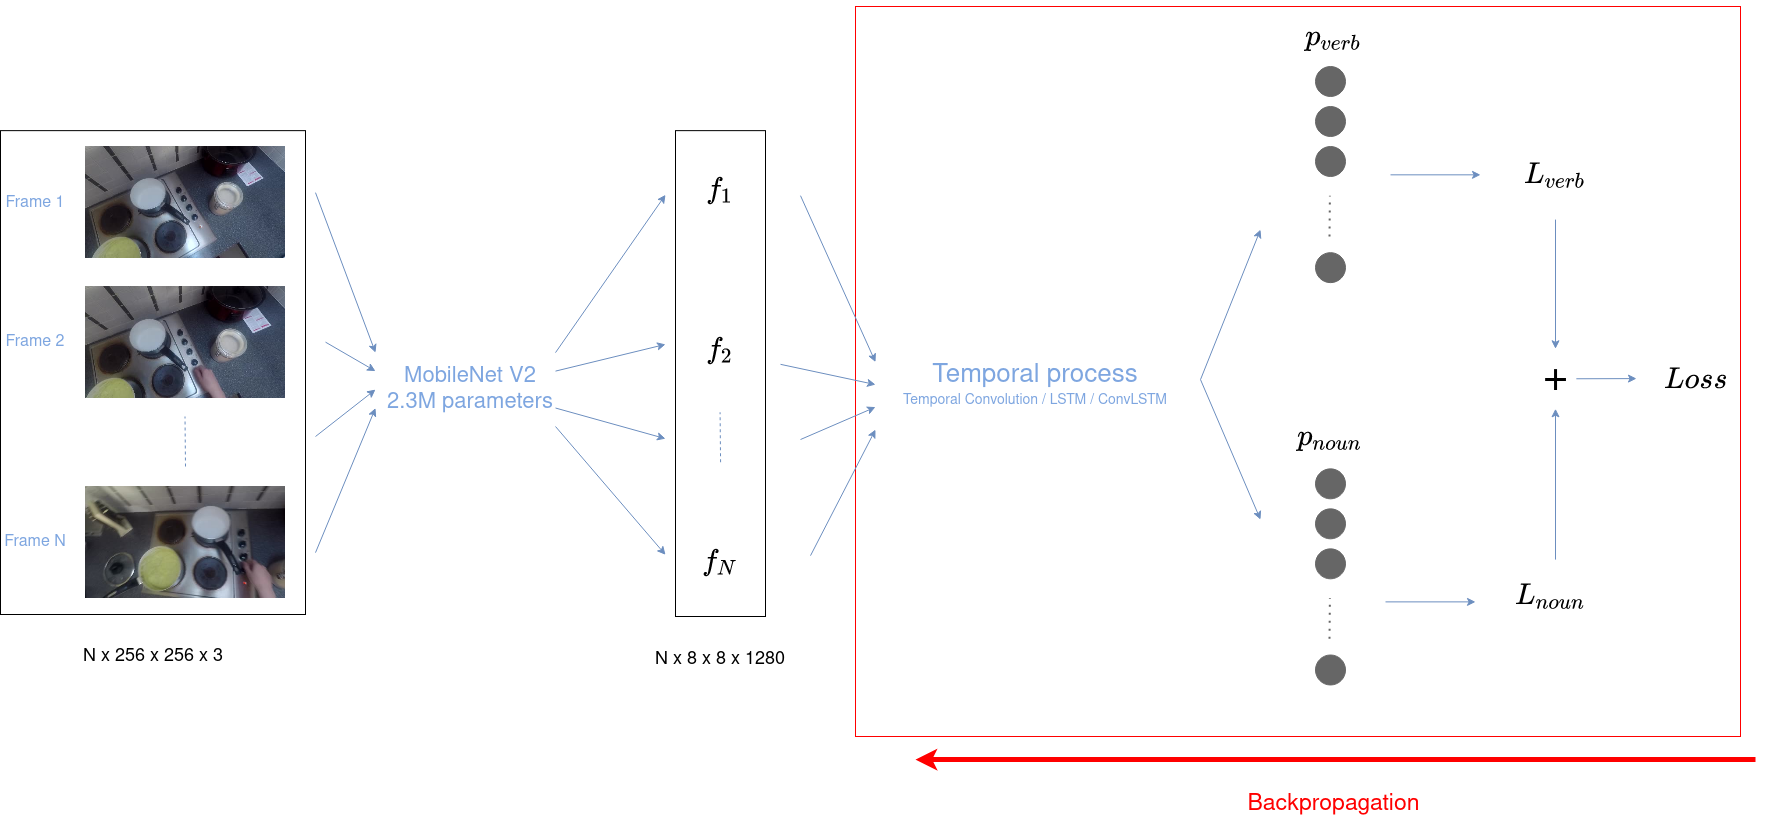
\includegraphics[width=1.2\textwidth]{architecture_diagr.png}\label{common_base}}
					\caption{Common base.}
				\end{figure}
				We use the cross-entropy error between predicted and ground-truth labels as error function.
				\begin{align*}
					L_{verb} = -\sum_{i} y^{verb}_{i}log(\hat{y}^{verb}_{i}) \\
					L_{noun} = -\sum_{i} y^{noun}_{i}log(\hat{y}^{noun}_{i}) \\
					Loss = L_{verb} + L_{noun} \\
				\end{align*}
				where $y$ and $\hat{y}$ are the ground-truth and model prediction respectively.
			\subsection{Temporal process subsystem}
				\subsubsection{LSTM}\label{lstm}
					Recurrent neural networks have been largely successfully applied to sequence-to-sequence prediction problems, especially in \gls{nlp} \cite{wu2016google,shen2018natural,miao2020application}.
					Their ability to propagate information during the inference is particularly appreciated as well as their independence of the sequence length, indeed the weights are shared across the sequence elements (which required the introduction of the {\itshape backpropagation through time} algorithm).
					They also attracted a lot of attention due to their ability to counter \gls{vanish}, especially LSTM \cite{Hochreiter1997lstm}; a brief recall of how RNN and LSTM work is described in appendix \ref{appendix_b}.
					Despite their success, LSTM are also known to encounter chaotic behaviour sometimes \cite{bertschinger2004,laurent2016recurrent}, which make them difficult to train with little data.
					Albeit these difficulties, we still tried to use LSTM because of its popularity.
					Nonetheless, we must ensure that what is fed to the LSTM is a sequence of vectors and not images.
					We thus used {\itshape global average pooling} on the output of MobileNetV2 to shrink them to vectors.
					Global average pooling is illustrated in Figure \ref{gap}, where $k$ is the mean filter with the same size as $A$.
					\begin{figure}[h!]
						\centering
						\subfloat{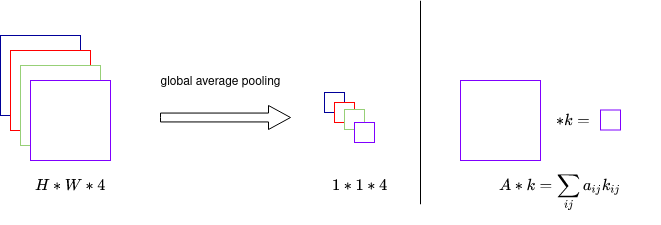
\includegraphics[width=0.9\textwidth]{gap.png}\label{gap}}
						\caption{Global average pooling.}
					\end{figure}
				\subsubsection{ConvLSTM}
					As mentioned in \ref{literature}, ConvLSTM were designed to counter the inability of LSTM to work with images.
					Indeed, LSTM works with vectors only, which constrain us to shrink the images (or feature maps) into vectors, wether by flattening or applying spatial pooling or feature extraction.
					However, these operations result in a loss of information, sometimes to the detriment of useful information.
					ConvLSTM is a good alternative that comes with all the potential of a CNN fused with the recurrence ability of LSTM.
					However, one must consider that by using images, we drastically augment the number of parameters needed in the ConvLSTM.
					As an example if we consider a sequence of $N*256*256$ RGB images going through MobileNetV2, we recover a sequence of $8*8$ feature maps with $1280$ channels each one.
					To send this through a LSTM, one must beforehand apply a spatial pooling to shrink those feature maps into $1*1$.
					This sequence of vectors ($N*1*1*1280 \Leftrightarrow N*1280$) is then fed to a LSTM which output a feature vector with, let's say, 50 features.
					This LSTM will then have ~266K parameters.
					If we do the same with a ConvLSTM, meaning we don't have to apply spatial average beforehand, that takes the $N*8*8*1280$ feature maps and use 50 kernels of size $4*4$ with a stride of 4 (as an example), it will result in an output of size $2*2*50$, thus requiring to apply spatial pooling before any fully connected layer; however applying spatial pooling on a $2*2$ result in less information loss than on $8*8$.
					This ConvLSTM will unfortunately have ~4.2M parameters, which is more than 15 times bigger than the LSTM, while both result in a feature vector of dimension 50.
					\begin{figure}[h!]
						\centering
						\subfloat[]{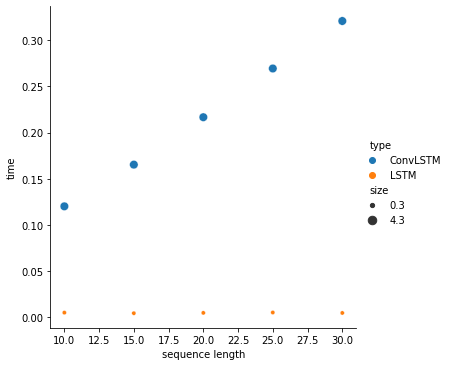
\includegraphics[width=0.47\textwidth]{compare_50.png}\label{comparison_50}}
						\hfill
						\subfloat[]{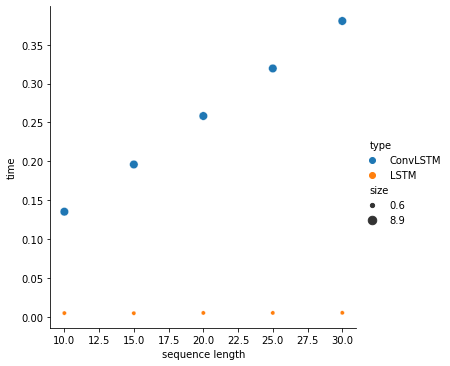
\includegraphics[width=0.47\textwidth]{compare_100.png}\label{comparison_100}}
						\vfill
						\subfloat[]{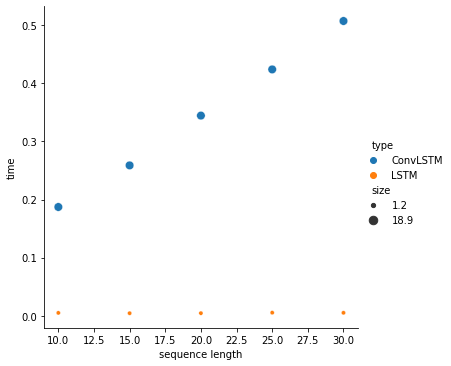
\includegraphics[width=0.47\textwidth]{compare_200.png}\label{comparison_200}}
						\hfill
						\subfloat[]{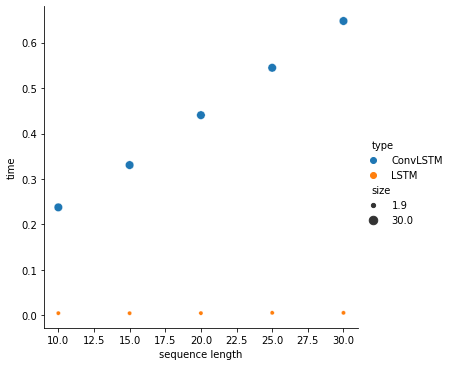
\includegraphics[width=0.47\textwidth]{compare_300.png}\label{comparison_300}}
						\caption{Comparison of differents aspects between LSTM and ConvLSTM.}
						\label{comparison}
					\end{figure}
					\par
					To compare them, we provide a graphical illustration, Figure \ref{comparison}, of different values such as:
					\begin{itemize}
						\item {\itshape time}: the time required to infer on one sample (milliseconds)
						\item {\itshape sequence length}
						\item {\itshape size}: number of parameters (rounded to the million)
					\end{itemize}
					The computations were done on Google Colab using an NVIDIA Tesla K80.
					The Figure \ref{comparison_50} represent the computation time as a function of the sequence length, sequences of $8*8*1280$ images (or feature maps), where the output dimension is 50.
					Figures \ref{comparison_100}, \ref{comparison_200} and \ref{comparison_300} are similar but with an output dimension of 100, 200, and 300 respectively.
					We can see that the advantage of the ConvLSTM over LSTM is rapidly taken over by the computation time and number of parameters to train.
					In our studies, we used a ConvLSTM layer with 8 kernels of size $4*4$.
					We also chosen to use a stride of 4, to avoid losing too much during the spatial pooling afterwards.
					\par
					Except for the convolutions, the internal structure of ConvLSTM is the same as LSTM (see appendix \ref{appendix_b}).
				\subsubsection{ConvNet1D}
					Before using these RNN architectures to manipulate time-series data, a different approach was to use 1D convolutions, also called {\itshape temporal convolutions}.
					It consists of taking a sequence of feature vectors and applying 1D convolutions.
					The kernel size of the convolution define the time window perceived by the convolution, i.e. how many seconds (or milliseconds) of the action the convolution is looking at.
					The advantage of temporal convolutions is the possibility to decompose the temporal processing in many depth levels.
					Rather than taking the kernel size being equal to the sequence length, which enforce it to extract the temporal correlations in one step, we can decompose the extraction in many depth levels as illustrated in Figure \ref{temp_conv}.
					On the left we have a 1 level deep temporal convolution which have to extract the temporal correlations in one convolution, whereas on the right we increase the depthness to construct a hierarchical extraction of the temporal correlations; notice that the circles are actually vectors here.
					\begin{figure}[h!]
						\centering
						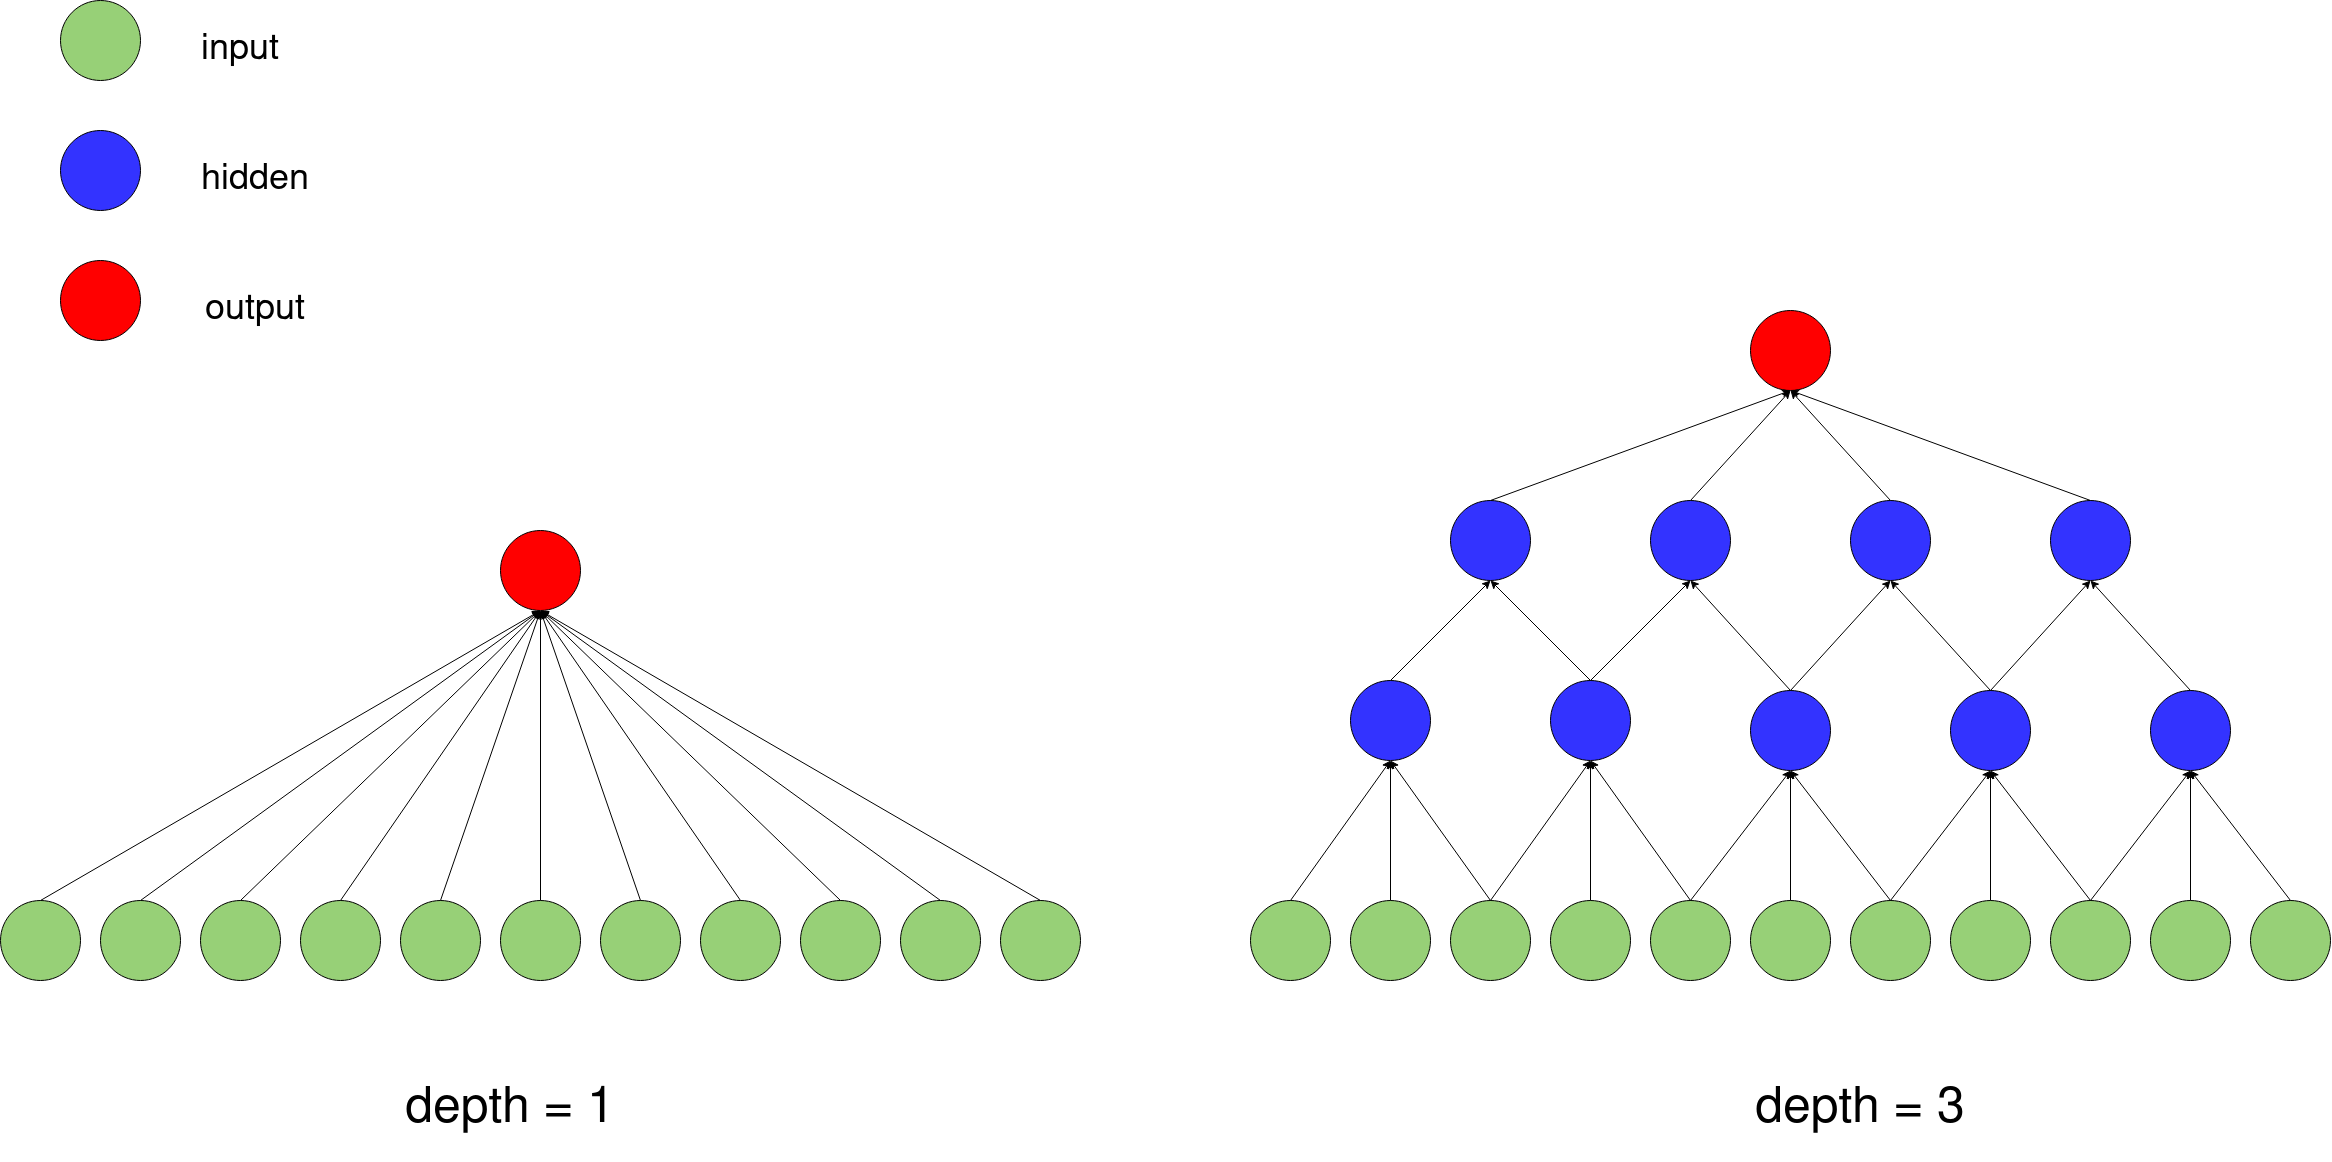
\includegraphics[width=0.8\textwidth]{temporal_convolution.png}
						\caption{Temporal convolutions of different depth.}\label{temp_conv}
					\end{figure}
					\par
					We use these temporal convolutions the same way we use a LSTM, i.e. the images go through MobileNetV2, then we retrieve the resulting feature maps, we apply some spatial pooling to shrink them to vectors, and feed the resulting feature vectors to a CNN of 1D convolutions.
					In our studies, this {\itshape ConvNet1D} consists of stacked 1D convolutions (using kernels of size 3) with batch normalization and LeakyReLU activation.
		\section{Results and interpretation}
			In a first attempt, we used EPIC-KITCHENS-55 to reduce the training time in order to explore the different possibilities in terms of: architecture, hyperparameters and data processing.
			All the models were trained using the Adam optimizer with an initial learning rate of 0.001 and a learning rate decay of 0.2 starting from epochs 35, every 20 epochs.
			We used different batchs sizes, depending on how much GPU were used and how much data were used.
			We also added a dropout of 0.5 before the two fully-connected layer to reduce overfitting.
		\section{Tools}
			It's almost frightening the ease with which one can implement deep learning algorithms.
			Back in the 90's, researchers would take several weeks to develop a simple ConvNet, and even more to train it.
			Today, with the python librairies, GPUs and storage devices that we have access to, such ConvNet can be written and train in hours only.
			The tools that we have in our disposition make deep learning looks like a children game, and may be dangerous if we use is without knowing what is under the hood.
			For this project we used the Keras API, that is built on Tensorflow (2.4), to develop, train and test our models, coupled with two NVIDIA GTX 1080Ti.
			We used distributed training to speed up the training because of the large size of one sample (i.e. a $N*256*256*3$, where $N$ can be up to 20).
			Indeed, this large size prevented us from loading all the dataset in memory and train the models in one stage, we were therefore forced to resort to a workaround described in section \ref{difficulties}.
		\section{Difficulties and problems}\label{difficulties}
			The major difficulty of this project was the memory management, for two reasons:
			\begin{itemize}
				\item Let's consider the size of one sample where the sequence length is fixed to 20: $20*256*256*3 = 3932160$. Each sample is a vector of almost 4 millions float32 values, which makes a total of 15Mo footprint for one such sample; a float32 value is encoded in 4 bytes.
				Considering that we had 250Go of RAM, it means that we can fit only 17K samples at a time, meanwhile our train set contained 67K samples.
				\item While a model was training using theoretically 30\% of the RAM, because we divided the dataset in this way, we realized that it was actually using more than 60\%.
				After some investigations we found that keras was storing a duplicate of the data in the backend resulting in a surplus of memory usage, with even memory leak at some point.
			\end{itemize}
			These two reasons forced us to take memory management under serious consideration.
			We decided to divide the training procedure by training the models on groups of data.
			We divide our training/validation data in groups such that each group size is equal to a certain percentage of the RAM.
			We load the first group and train the model for a certain number of epochs and we record some validation metrics.
			We then do the same thing for each other groups until all the model get through all of them.
			At this point we go back to the frist group and iterate until all groups have been used $n$ times; where $n$ is the number of epochs.
	\chapter{Conclusion}
		\section{Results synthesis}
			Lorem ipsum.
		\section{Observations}
			Lorem ipsum.
		\section{Roads for investigation}
			Lorem ipsum.
		\section{Acquired knowledge and skills}
			Lorem ipsum.
	\bibliographystyle{apalike}
	\bibliography{bibliography}
	\appendix
	\chapter{ImageNet and EPIC-KITCHENS comparisons}\label{appendix_a}
		\begin{figure}[h!]
			\centering
			\subfloat[EPIC-KITCHENS]{
				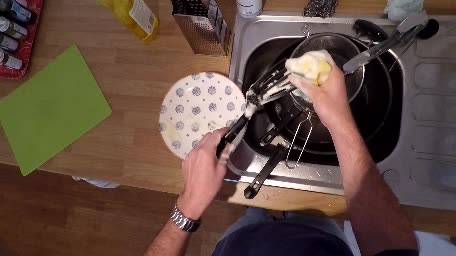
\includegraphics[width=0.3\textwidth]{epickitchens1.jpg},
				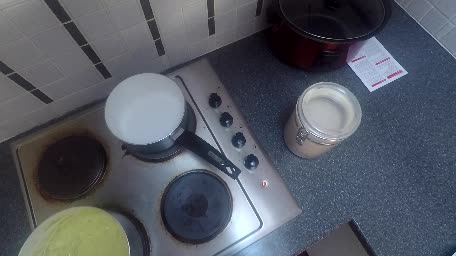
\includegraphics[width=0.3\textwidth]{epickitchens2.jpg},
				
\includegraphics[width=0.3\textwidth]{epickitchens3.jpg}}
			\hfill
			\subfloat[ImageNet]{
				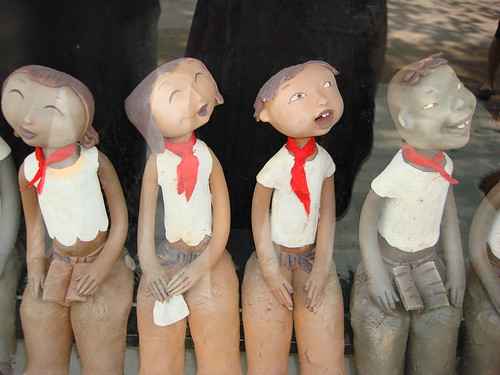
\includegraphics[width=0.3\textwidth]{imagenet1.jpeg},
				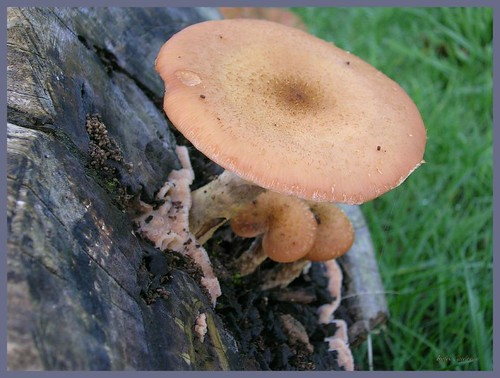
\includegraphics[width=0.3\textwidth]{imagenet2.jpeg},
				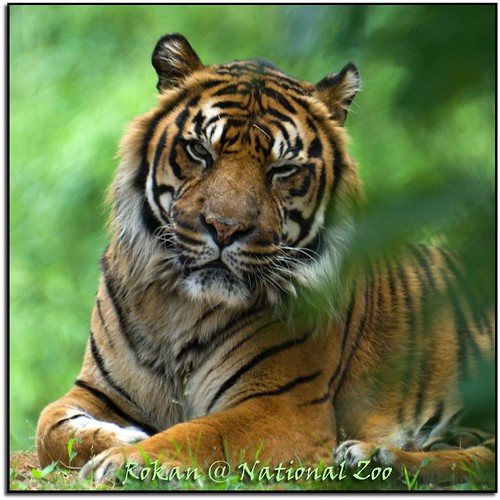
\includegraphics[width=0.3\textwidth]{imagenet3.jpeg}}
		\end{figure}
	\chapter{Reccurent Neural Networks / Long-Short Term Memory}\label{appendix_b}
		Processing time-sequence data with deep architectures has been challenging due to the necessity of incorporating a memory mechanism.
		To handle this, Recurrent Neural Network (RNN) use a recursive loop over the sequence elements while maintaining a memory state called {\itshape hidden state} reffered as {\itshape $a^{<>}$} in Figure \ref{rnn}.
		This hidden state is charged to keep information flowing through the network by being updated at every step.
		\begin{figure}[h!]
			\centering
			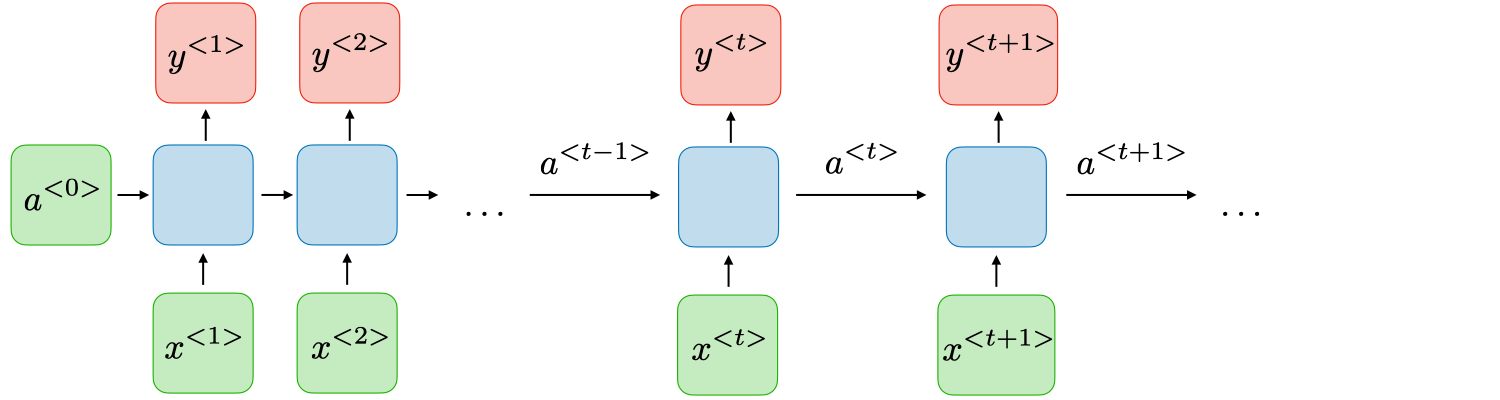
\includegraphics[width=1.\textwidth]{architecture-rnn-ltr.png}
			{\tiny \url{https://stanford.edu/~shervine/teaching/cs-230/cheatsheet-recurrent-neural-networks}}
			\caption{vanilla RNN architecture.}
			\label{rnn}
		\end{figure}
		A RNN cell, depicted in Figure \ref{rnn_cell}, uses {\itshape gates} to encode, update and reset information; the learnable weights are ({\itshape $W_{aa},W_{ax},W_{ya},b_{a},b_{y}$}).
		\begin{figure}[h!]
			\centering
			\subfloat[vanilla RNN cell.]{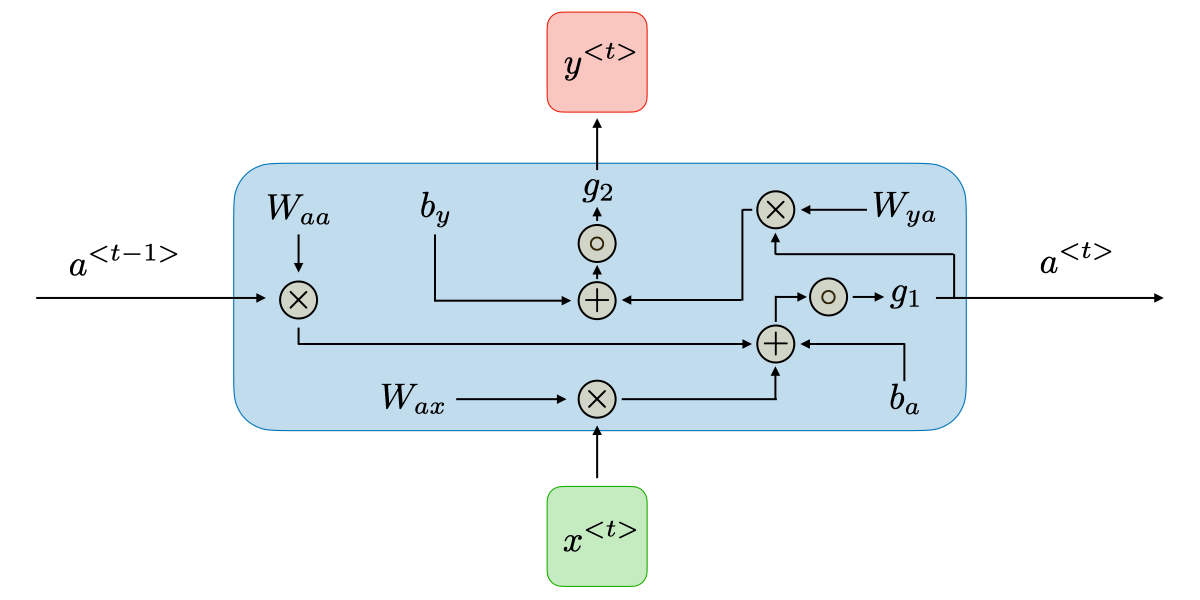
\includegraphics[width=0.55\textwidth]{description-block-rnn-ltr.png}\label{rnn_cell}}
			\hfill
			\subfloat[LSTM cell.]{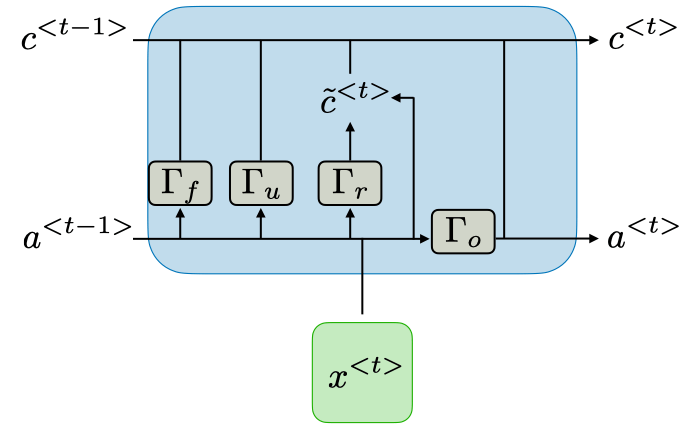
\includegraphics[width=0.4\textwidth]{lstm-ltr.png}\label{lstm_cell}} \\
			{\tiny \url{https://stanford.edu/~shervine/teaching/cs-230/cheatsheet-recurrent-neural-networks}}
			\caption{Recurrent cells description.}
		\end{figure}
		\par
		A successful implementation of RNN is called Long Short-Term memory \cite{Hochreiter1997lstm}.
		Its particularity is that it implements not one but two states called {\itshape hidden} ($a_{t}$) and {\itshape cell} ($c_{t}$) states.
		The purpose of the cell state in LSTM is to allow for long-term dependencies, inducing a long-term memory.
		While their memory cell are more complex than RNN's, see Figure \ref{lstm_cell}, they exhibit most of the time better performance due to their ability to catch these long-term dependencies.
		The flow of information through the cell state, top line of Figure \ref{lstm_cell}, has been shown to help counter gradient vanishing.
		\par
		LSTM equations:
		\begin{align*}
			& \Gamma_{f} = \sigma(W_{f}x_{t} + U_{f}a_{t-1} + b_{f}) \\
			& \Gamma_{u} = \sigma(W_{u}x_{t} + U_{u}a_{t-1} + b_{u}) \\
			& \Gamma_{r} = \sigma(W_{r}x_{t} + U_{r}a_{t-1} + b_{r}) \\
			& \Gamma_{o} = \sigma(W_{o}x_{t} + U_{o}a_{t-1} + b_{o}) \\
			& \tilde{c}_{t} = tanh(W_{c}[\Gamma_{r} \circ a_{t-1},x_{t}] + b_{c}) \\
			& c_{t} = \Gamma_{f} \circ c_{t-1} + \Gamma_{u} \circ \tilde{c}_{t} \\
			& a_{t} = \Gamma_{o} \circ tanh(c_{t})
		\end{align*}
		where $\sigma$ is the sigmoid activation function, $tanh$ the hyperbolic tangent function, $\circ$ denotes the Hadamard or element-wise product and the learnable weights (and biases) are $W$, $U$ and $b$.
		($\Gamma_{f}$, $\Gamma_{u}$, $\Gamma_{r}$, $\Gamma_{o}$) are the LSTM gates and their purpose is to forget, update, reset and reveal the information respectively.
		At the first step, $c_{0}$ and $a_{0}$ are set to 0.
	\chapter{Optical Flow fields}\label{appendix_c}
		We provide some examples of visualization of optical flow between two RGB images ($I_{1}$ and $I_{2}$).
		For this we have to understand that (dense) optical flows are per-pixel motion estimation, which result to an horizontal and vertical motions.
		Thus, they are computed as an horizontal, called {\itshape u}, and vertical, called {\itshape v}, displacements.
		To combine these two, we can computes the magnitude of the optical flow field, which is $m = \sqrt{u^{2} + v^{2}}$.
		All of these are shown in Figure \ref{optical_flow}.
		\begin{figure}[h!]
			\centering
			\subfloat[$I_{1}$]{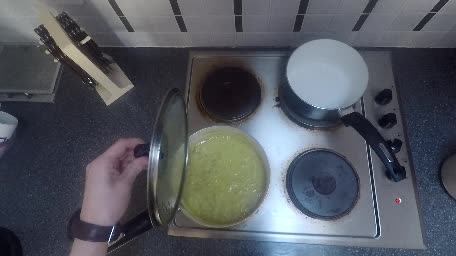
\includegraphics[width=0.35\textwidth]{opticalflow/rgb1.png}}
			\hfill
			\subfloat[$I_{2}$]{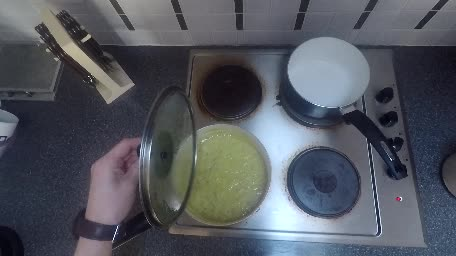
\includegraphics[width=0.35\textwidth]{opticalflow/rgb2.png}}
			\vfill
			\subfloat[$u$]{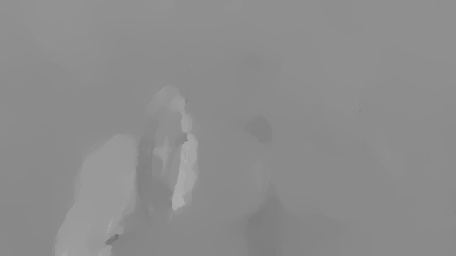
\includegraphics[width=0.35\textwidth]{opticalflow/u.jpg}}
			\hfill
			\subfloat[$v$]{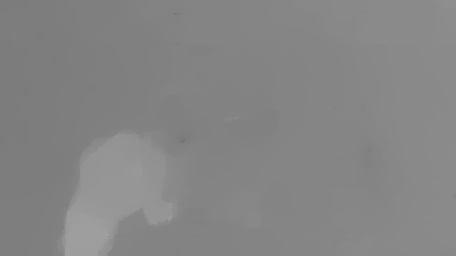
\includegraphics[width=0.35\textwidth]{opticalflow/v.jpg}}
			\vfill
			\subfloat[$m$]{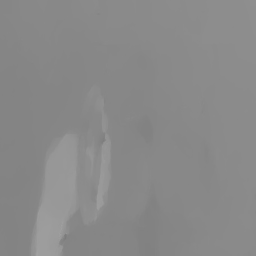
\includegraphics[width=0.3\textwidth]{opticalflow/uv.png}}
			\caption{Optical flow field example.}\label{optical_flow}
		\end{figure}
	\makeutbmbackcover{}
\end{document}
